\subsection{\texttt{undl}: A Python library to wrap to the UN Digital Library API} \label{ssec:undl-a-python-library-to-wrap-to-the-un-digital-library-api}

For the \texttt{undl} library, I used Python 3.10 with packages, with \texttt{requests} for the HTTP requests, \texttt{pandas} for the data manipulation, and \texttt{pydantic} for the data validation.

Its purpose is to query the UN Digital Library API, and to return the results in a structured way and convenient way. It converts the \texttt{MARCXML} response from the API to a \texttt{JSON} object and implements caching to save the results of the queries, and to avoid querying the API again if the same query is made. The client offers these main methods:

\begin{itemize}
    \item \texttt{query(...)}:
          Takes the prompt (e.g., \texttt{"Women in peacekeeping"}) as an argument, and returns the detailed results of the query as a \texttt{JSON} object. The API response is a list of detailed documents (the fields we actually collect are precised in \ref{ssec:neo4j-graph-database} for the \texttt{Document} node type).
          The main difference with a direct call to the UNDL API is that it converts the output to a \texttt{JSON} object. It is used by \repo{un-semun-api} (\ref{ssec:un-semun-api-an-api-for-un-semun-front-using-fastapi}).

    \item \texttt{getAllRecordIds(...)}:
          Same as \texttt{query}, but returns only the IDs of the documents, not their entire fields - hence is much faster. It is used by \repo{un-semun-api} (\ref{ssec:un-semun-api-an-api-for-un-semun-front-using-fastapi}) and \repo{un-ml-pipeline} (\ref{ssec:un-ml-pipeline-the-machine-learning-pipeline}).

    \item \texttt{queryBdId(...)}:
          Queries the API for a single document, given its \texttt{id}. It is used by \repo{un-ml-pipeline} (\ref{ssec:un-ml-pipeline-the-machine-learning-pipeline}).
\end{itemize}

These methods are callable either from the command-line interface (CLI), or from another Python script when imported as a library (see an example in Figure \ref{fig:undl-py})

\begin{figure}[!ht]
    \centering
    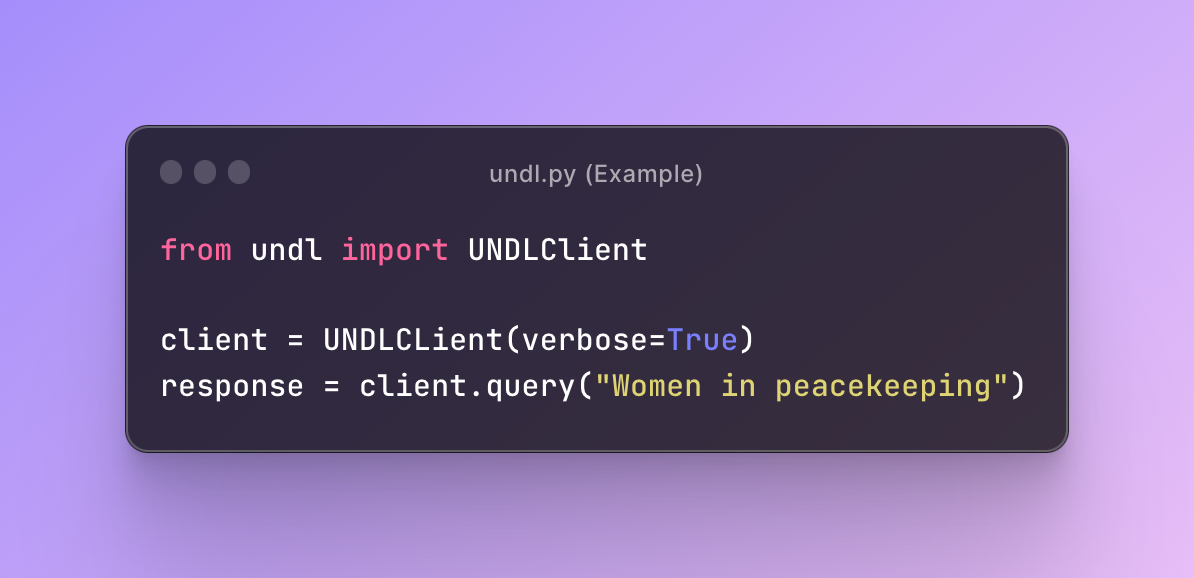
\includegraphics[width=0.6\textwidth]{res/import-undl.png}
    \caption{Querying the UNDL API from a Python script using \texttt{undl} library}
    \label{fig:undl-py}
\end{figure}

Note that \texttt{undl} requires a valid UNDL API key to work (set using the environment variable \texttt{UN\_API}), because the API calls are authenticated by this $36$ characters long key.
